\section{Results}
\label{sec:results}

\begin{figure}[!t]
\centering
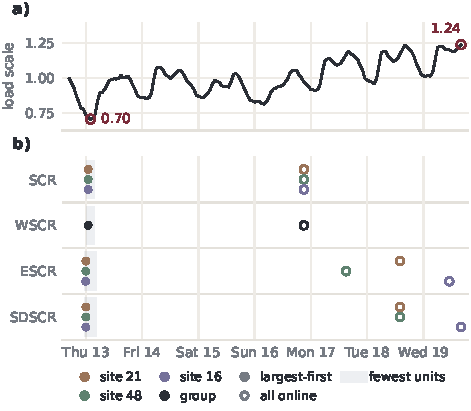
\includegraphics[width=\linewidth]{f2_week}
\caption{Intact week. (a) Load scale, with the minimum- and peak-load hours. (b) Hour at which
each metric is lowest at each site, under the largest-first rule (filled) and with every unit
online (open); minimum-commitment hours shaded.}
\label{fig:week}
\end{figure}

\subsection{When each site is weakest}

Under the largest-first rule, commitment follows load (Fig.~\ref{fig:week}): the fewest units
are online around the minimum-load hour, and commitment never falls as load rises. The results
are counted over ten metric--site pairs, three sites each for SCR, ESCR and SDSCR and one group
value for WSCR, and over \NumCases{} cases, the intact network and the \NumCorridors{} corridors. The
weekly minimum falls in these minimum-commitment hours in \NumConeAll{} pair--case
combinations (Fig.~\ref{fig:week}b). The cause is the driving-point impedance: with fewer
generators committed, fewer source admittances lie in parallel and $|Z_{ii}|$ rises. With $\delta_Z$ isolated
in~\eqref{eq:split} ($\delta_V$ and $\delta_I$ set to zero), every combination has its weakest
hour in these hours. The
\NumConeExceptions{} exceptions, all SCR or WSCR under outages, are combinations in which the change in the pre-fault voltage $\delta_V$
slightly outweighs the change in the driving-point impedance $\delta_Z$ in~\eqref{eq:split}.

With every unit online throughout the intact week, commitment no longer changes and the weakest hour moves to high load, at
load scales of \NumCtwoLoadLow{} to \NumCtwoLoadHigh. The pre-fault voltage falls as load rises,
and in every pair $\delta_V$ outweighs $\delta_Z$ in~\eqref{eq:split}. The driving-point
impedance changes only through the loads, which the fault model represents as constant
impedances (Section~\ref{sec:metrics}-A), so with $\delta_Z$ isolated the weakest hour would be at
minimum load (hour \NumCtwoZonlyHour). From that hour to the actual weakest hour, however, the
voltage part reduces the metric ($\delta_V$ from \NumCtwoDeltaVLow{} to \NumCtwoDeltaVHigh) more than the impedance part
raises it ($\delta_Z$ from \NumCtwoDeltaZLow{} to \NumCtwoDeltaZHigh). The metrics then vary much less: each pair's weekly maximum exceeds its
minimum by \NumCtwoRangeLow{} to \NumCtwoRangeHigh, against \NumConeRangeLow{} to
\NumConeRangeHigh{} under the largest-first rule. Their weakest hours, however, spread over
\NumCfourSpanEfive, within which each metric rises by a median of \NumCfourWindowMedian{} above
its weekly minimum (at most \NumCfourWindowMax, \NumCfourWindowMaxMetric). With commitment
fixed, the metrics thus disagree on the weakest hour.

Commitment thus sets the weakest hour wherever it varies, and otherwise the pre-fault voltage does, though the metrics then vary far less over the week.
This also explains the planning snapshots. Under the largest-first rule the
minimum-load hour is a minimum-commitment hour, and its snapshot lies within
\NumCthreeGapEone{} of the true minimum. With every unit online, the minimum-load snapshot
misses the true minimum by up to \NumCthreeGapEfiveMin.

\begin{figure*}[!t]
\centering
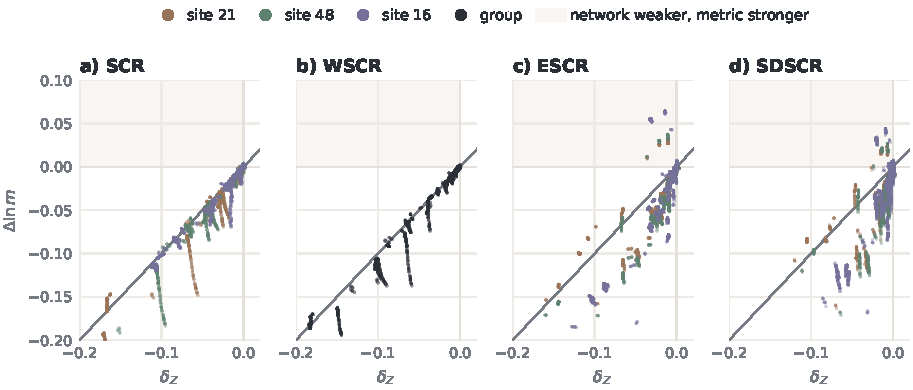
\includegraphics[width=\textwidth]{f3_outage}
\caption{Change $\Delta\ln m$ of each metric under a branch outage against its
driving-point-impedance part $\delta_Z$ in~\eqref{eq:split}, per point: (a) SCR, (b) WSCR,
(c) ESCR, (d) SDSCR. Shaded: network weaker, metric stronger. Points below $-0.2$ are not drawn (\NumFthreeBeyondSCR,
\NumFthreeBeyondWSCR, \NumFthreeBeyondESCR{} and \NumFthreeBeyondSDSCR{} points; lowest
\NumFthreeLowestSCR, SCR).}
\label{fig:outage}
\end{figure*}

\subsection{What a branch outage does}

Results under outages are counted per point, one corridor, hour and site: \NumPoints{} points per
metric, and \NumPointsGroup{} for the WSCR group value. An outage weakens the network or leaves it practically unchanged: $\delta_Z$ never exceeds
\NumCfiveDeltaMax{} (\NumCfiveNetMax), while it reaches \NumCfiveDeltaMin{} (\NumCfiveNetMin) at
worst. Fig.~\ref{fig:outage} plots each metric's change against this network change.
SCR and WSCR follow it, with no point more
than 1\,\% stronger; their points below the diagonal are those in which the pre-fault voltage
falls as well. ESCR and SDSCR follow it less closely and occasionally oppose it:
\NumCsevenOppESCR{} and \NumCsevenOppSDSCR{} points (\NumCsevenShareESCR{} and
\NumCsevenShareSDSCR) are more than 1\,\% stronger while
the network weakens, by at most \NumCsevenMaxESCR{} and \NumCsevenMaxSDSCR. 
All such points come from outages of a line at another plant's POI. The outage moves that plant
electrically away from the site, so its interaction factor falls and $\delta_I$ outweighs
$\delta_Z$ in~\eqref{eq:split}.
With $\delta_I$ set to zero, no point remains more than 1\,\% stronger, while with $\delta_V$ set to zero they remain. The
opposition thus comes from the interaction term in the metrics' definitions, not from a
convention.

\begin{figure}[!t]
\centering
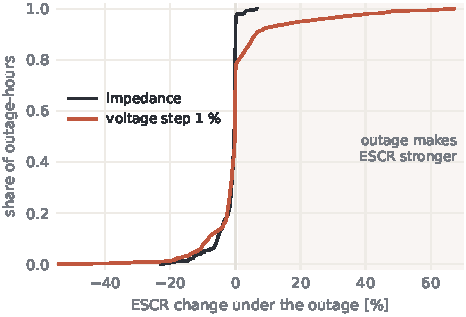
\includegraphics[width=\linewidth]{f4_interaction_factor}
\caption{Cumulative share of points by ESCR's change under an outage, with the
impedance-based interaction factor and the 1\,\% voltage step with generators regulating.
Shaded: more than 1\,\% stronger.}
\label{fig:miif}
\end{figure}

\subsection{How the interaction factor changes ESCR}

Fig.~\ref{fig:miif} compares ESCR's outage change under the impedance-based interaction factor
and under the 1\,\% voltage step. With the impedance form, ESCR is more than 1\,\%
stronger in \NumCsevenShareESCR{} of the points, as found in Section~\ref{sec:results}-B. With the
1\,\% voltage step, the share rises to \NumCeightProbeOneShare, and ESCR is up to \NumCeightProbeOneMax{}
stronger.
Using steps of 0.5 and 2\,\%, the share is \NumCeightProbeHalfShare{} and \NumCeightProbeTwoShare. A likely cause is the generators' voltage control. In
the voltage step, generators that regulate their terminal voltages hold the voltage near the
other plants, so $\Delta V_j$, and with it $\mathrm{MIIF}_{ji} = \Delta V_j/\Delta V_i$, is smaller
than in the impedance form, which contains no such response. $D_i$ then falls and ESCR rises. ESCR's response to
outages thus depends on how its interaction factor is obtained.
